% !TeX encoding = UTF-8
% !TeX spellcheck = pl_PL



% $Id:$

%Author: Wojciech Domski
%Szablon do ząłożeń projektowych, raportu i dokumentacji z steorwników robotów
%Wersja v.1.0.0
%


%% Konfiguracja:
\newcommand{\kurs}{Sterowniki robot\'{o}w}
\newcommand{\formakursu}{Projekt}

%odkomentuj właściwy typ projektu, a pozostałe zostaw zakomentowane
\newcommand{\doctype}{Za\l{}o\.{z}enia projektowe} %etap I
%\newcommand{\doctype}{Raport} %etap II
%\newcommand{\doctype}{Dokumentacja} %etap III

%wpisz nazwę projektu
\newcommand{\projectname}{Humanistycznie upo\'sledzony robot akrobatyczny}

%wpisz akronim projektu
\newcommand{\acronim}{HURA}

%wpisz Imię i nazwisko oraz numer albumu
\newcommand{\osobaA}{Albert \textsc{Lis}, 235534}
%w przypadku projektu jednoosobowego usuń zawartość nowej komendy
\newcommand{\osobaB}{Micha\l{} \textsc{Moru\'n}, 235986}

%wpisz termin w formie, jak poniżej dzień, parzystość, godzina
\newcommand{\termin}{sr TP15 }

%wpisz imię i nazwisko prowadzącego
\newcommand{\prowadzacy}{mgr in\.{z}. Wojciech \textsc{Domski}}

\documentclass[10pt, a4paper]{article}
\usepackage[utf8]{inputenc}
\usepackage{polski}
\usepackage[usenames,dvipsnames]{xcolor}

%Preambuła dokumentu

% linki w spisie tresci, bibliografi
\usepackage[bookmarks=true,bookmarksnumbered=false,unicode=true,pdftex=true, colorlinks,filecolor=black,linkcolor=black,urlcolor=black,citecolor=black]{hyperref}

%ustawienie rozmiaru papieru
\usepackage[a4paper, left=2.5cm, right=2.5cm, top=2.5cm, bottom=2.5cm, headsep=1.2cm]{geometry}

%rozmaite ustawienia pozwalające okreslić język

%NALEŻY wybrać jeden z pakietów
%\usepackage{polski} %przydatne podczas składania dokumentów w j. polskim
\usepackage[polish]{babel}  % pakiet lokalizujący dokument w języku polskim
%\usepackage[british]{babel}

\usepackage{indentfirst}	% polski styl pisania (np. rozpoczecie pierwszego akapitu
% pod nazwa rozdzialu od wciecia)
%\usepackage[OT4]{fontenc}
\usepackage[utf8]{inputenc} % w miejsce utf8 można wpisać latin2 bądź cp1250,
% w zależności od tego w jaki sposób kodowane są 
% polskie znaki diakrytyczne przy wprowadzaniu 
% z klawiatury.
%kodowanie znaków, zależne od systemu
\usepackage[T1]{fontenc} %poprawne składanie polskich czcionek

%OPEROWANIE NA OBRAZACH
\usepackage{graphicx}       % pakiet graficzny, umożliwiający m.in.
% import grafik w formacie eps
%\usepackage{epstopdf}		% pozwala na importowanie grafik w formacie eps
% przy użyciu pdflatex
\usepackage[update,prepend]{epstopdf}
\usepackage{rotating}       % pakiet umożliwiający obracanie rysunków
\usepackage{subfigure}      % pakiet umożliwiający tworzenie podrysunków
\usepackage{epic}           % pakiet umożliwiający rysowanie w środowisku latex
\usepackage{psfrag}         % pakiet umożliwiający podmianę łańcuchów znaków 
% w plikach eps
%\usepackage{curves}         % pakiet do wykreslania krzywych

%pakiety dodające dużo dodatkowych poleceń matematycznych
\usepackage{amsfonts}       % pakiet z rozmaitymi czcionkami matematycznymi
%\usepackage{amssymb}        % pakiet z rozmaitymi symbolami matematycznymi
\usepackage{amsmath}        % pakiet z rozmaitymi środowiskami matematycznymi

\usepackage{fp}             % pakiet z funkcjami operujacymi 
% na liczbach zmiennoprzecinkowych
\usepackage{calc}           % pakiet umożliwiający operacje arytmetyczne
% na tzw. licznikach (liczbach całkowitych)
\usepackage{leftidx}		% indeksy górne i dolne po lewej stronie

%definicje matematyczne
\providecommand{\abs}[1]{\lvert#1\rvert}
\providecommand{\norm}[1]{\lVert#1\rVert}

%pakiety wspomagające i poprawiające składanie tabel
\usepackage{supertabular}
\usepackage{array}
\usepackage{tabularx}
\usepackage{hhline}
\usepackage{longtable}		% wsparcie dla dlugich tabel
\usepackage{multicol}		% podzial strony na wiele kolumn

%pakiet do BibTex
\usepackage{cite}

\usepackage{url} %pakiet pozawalający na dodawanie adresów url w bibliografi

%pakiet wypisujący na marginesie etykiety równań i rysunków zdefiniowanych przez \label{}, chcąc wygenerować finalną wersję dokumentu wystarczy usunąć poniższą linię
%\usepackage{showlabels}

\usepackage{float}			% lepsza obsluga mechanizmow obiektow plywajacych
% wymuszenie wstawienia np. tabeli, obrazka w danym miejscu przez [H]

\usepackage{listings}       % pakiet dedykowany zrodlom programow
\usepackage{color}


\definecolor{dkgreen}{rgb}{0,0.6,0}
\definecolor{gray}{rgb}{0.5,0.5,0.5}
\definecolor{mauve}{rgb}{0.58,0,0.82}

\lstset{ %
	language=C,                % the language of the code
	basicstyle=\small,           % the size of the fonts that are used for the code
	numbers=left,                   % where to put the line-numbers
	numberstyle=\footnotesize\color{gray},  % the style that is used for the line-numbers
	stepnumber=1,                   % the step between two line-numbers. If it's 1, each line 
	% will be numbered
	numbersep=5pt,                  % how far the line-numbers are from the code
	backgroundcolor=\color{white},      % choose the background color. You must add \usepackage{color}
	showspaces=false,               % show spaces adding particular underscores
	showstringspaces=false,         % underline spaces within strings
	showtabs=false,                 % show tabs within strings adding particular underscores
	%frame=single,                   % adds a frame around the code
	rulecolor=\color{black},        % if not set, the frame-color may be changed on line-breaks within not-black text (e.g. comments (green here))
	tabsize=2,                      % sets default tabsize to 2 spaces
	captionpos=b,                   % sets the caption-position to bottom
	breaklines=true,                % sets automatic line breaking
	breakatwhitespace=false,        % sets if automatic breaks should only happen at whitespace
	%title=\lstname,                   % show the filename of files included with \lstinputlisting;
	% also try caption instead of title
	keywordstyle=\color{blue},          % keyword style
	commentstyle=\color{dkgreen},       % comment style
	stringstyle=\color{mauve},         % string literal style
	escapeinside={\%*}{*)},            % if you want to add LaTeX within your code
	morekeywords={*,...},              % if you want to add more keywords to the set
	deletekeywords={...}              % if you want to delete keywords from the given language
}

%polish signs in lst code
\lstset{literate=%
	{ą}{{\k{a}}}1
	{ć}{{\'c}}1
	{ę}{{\k{e}}}1
	{ł}{{\l}}1
	{ń}{{\'n}}1
	{ó}{{\'o}}1
	{ś}{{\'s}}1
	{ż}{{\.z}}1
	{ź}{{\'z}}1
	{Ą}{{\k{A}}}1
	{Ć}{{\'C}}1
	{Ę}{{\k{E}}}1
	{Ł}{{\L}}1
	{Ń}{{\'N}}1
	{Ó}{{\'O}}1
	{Ś}{{\'S}}1
	{Ż}{{\.Z}}1
	{Ź}{{\'Z}}1
}

\usepackage{verbatim}       % pakiet dedykowany rozmaitym wydrukom tekstowym
\usepackage{ifthen}         % pakiet umożliwiający tworzenie prostych programów
% (m.in. zawiera instrukcje powtórzeniowe 
% i warunkowe)
\usepackage{upquote}		%normal quotations marks ' and `

% deklaracje wymagane przez pakiet theorem automatycznie ladowany w przypadku
% klasy dokumentu article
%
\newtheorem{Dn}{Definicja}[section]     % deklaracja srodowiska definicja
\newtheorem{La}[Dn]{Lemat}                % deklaracja srodowiska lemat
\newtheorem{Tm}[Dn]{Twierdzenie}          % deklaracja srodowiska twierdzenie
\newtheorem{Rk}[Dn]{Spostrze{\.z}enie}  % deklaracja srodowiska spostrzezenie
\newtheorem{Am}[Dn]{Algorytm}           % deklaracja srodowiska algorytm
\newtheorem{As}[Dn]{Za{\l}o{\.z}enie}   % deklaracja srodowiska zalozenie
\newtheorem{Pn}[Dn]{Propozycja}           % deklaracja srodowiska propozycja
\newtheorem{Py}[Dn]{W{\l}asno{\'s}{\'c}}  % deklaracja srodowiska wlasnosc
\newtheorem{Cy}[Dn]{Wniosek}              % deklaracja srodowiska wniosek
\newtheorem{Ee}[Dn]{Przyk{\l}ad}        % deklaracja srodowiska przyklad
\newtheorem{Ex}{{\'C}wiczenie}          % deklaracja srodowiska cwiczenie

%helps to specify width of a column in table
%\begin{tabular}{|C{1cm}|c|c|c|c|c|c|c|c|c|c|}
%first column will have widht of 1cm
\newcolumntype{L}[1]{>{\raggedright\let\newline\\\arraybackslash\hspace{0pt}}m{#1}}
\newcolumntype{C}[1]{>{\centering\let\newline\\\arraybackslash\hspace{0pt}}m{#1}}
\newcolumntype{R}[1]{>{\raggedleft\let\newline\\\arraybackslash\hspace{0pt}}m{#1}}

\sloppy			%zawija bardzo długie linie

%\pagenumbering{gobble}% Remove page numbers (and reset to 1)
	
\begin{document}

\def\tablename{Tabela}	%zmienienie nazwy tabel z Tablica na Tabela

\begin{titlepage}
	\begin{center}
		\textsc{\LARGE \formakursu}\\[1cm]		
		\textsc{\Large \kurs}\\[0.5cm]		
		\rule{\textwidth}{0.08cm}\\[0.4cm]
		{\huge \bfseries \doctype}\\[1cm]
		{\huge \bfseries \projectname}\\[0.5cm]
		{\huge \bfseries \acronim}\\[0.4cm]
		\rule{\textwidth}{0.08cm}\\[1cm]
		
		\begin{flushright} \large
		\emph{Skład grupy:}\\
		\osobaA\\
		\osobaB\\[0.4cm]
		
		\emph{Termin: }\termin\\[0.4cm]

		\emph{Prowadzący:} \\
		\prowadzacy \\
		
		\end{flushright}
		
		\vfill
		
		{\large \today}
	\end{center}	
\end{titlepage}

\newpage
\tableofcontents
\newpage

%Obecne we wszystkich dokumentach
\textcolor{Red}{To musi się znaleźć:} \newline
\textcolor{Red}{k1 in [0,1.0] — poprawne opracowanie dokumentu w systemie składania tekstu LaTeX, wykorzystanie dostarczonego szablonu \newline
	k2 in [0,0.5] — przynajmniej dwie pozycje literaturowe traktujące o problematyce projektu \newline
	k3 in [0,0.5] — przynajmniej 2 pozycje ściśle związane z wykorzystanym sprzętem, układami elektronicznymi,  modułami, itp.\newline
	k4 in [0,1.5] — merytoryczna część założeń projektowych \newline
	k5 in [0,0.5] — podział prac w projekcie na zadania.\newline}
\section{Opis projektu}
\label{sec:OpisProjektu}

Celem projektu jest zbudowanie zdalnie sterowanego robota jezdnego. Robot będzie sterowany za pomocą akcelerometru w telefonie. Dane będą przesyłanie za pomocą Wi-Fi lub Bluetooth. Regulacja prędkości będzie się odbywać za pomocą regulatora PID. Dane o prędkości będą pobierane z enkoderów znajdujących się w kołach robota. Opcjonalnie robot będzie wyświetlał szczegółowe dane o swoim stanie wewnętrznym za pomocą wbudowanego w płytkę z mikrokontrolerem wyświetlacza LCD.
\newline
\newline

\begin{figure}[H]
	\centering
	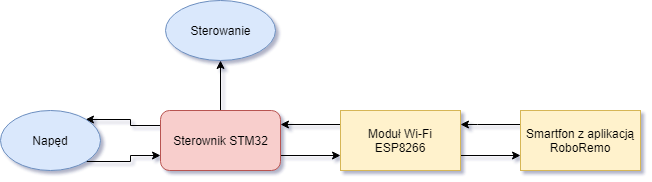
\includegraphics[width=0.8\textwidth]{figures/diagram.png}
	\caption{Architektura systemu}
	\label{fig:Architektura}
\end{figure}

\section{Założenia projektowe}

	\subsection{Mechanika}
	\begin{enumerate}
		\item Napęd
		\newline
		Napęd będzie realizowany na tylną oś za pomocą silnika szczotkowego DC. Regulacja prędkości oparta o regulator PID oraz sterowanie PWM.
		
		\item Sterowanie
		\newline
		Skręcanie będzie oparte o serwomechanizm. Serwomechanizm realizuje skręt przednich kół za pomocą poprzecznej belki przymocowanej do kół.
		
		\item Rama
		\newline
		Rama zbudowana z klocków lego. Posiada duże możliwości dopasowania do zmian w trakcie projektu.
	\end{enumerate}

	\subsection{Elektronika}
	\begin{enumerate}
		\item Mikrokontroler
		\newline
		Sterownik dostarczony przez prowadzącego STM32L476GDiscovery.
		
		\item Pomiar prędkości
		\newline
		Realizowany za pomocą enkoderów znajdujących się w kołach robota.
		
		\item Zasilanie
		\newline
		Oparte o akumulatory li-ion 18650 lub powerbank. Dopasowanie napięcia za pomocą przetwornicy step-up MT3608 do napędu kół oraz step-down do zasilania mikrokontrolera i modułu Wi-Fi w standardzie 3.3V.
	\end{enumerate}

	\subsection{Komunikacja}
	\begin{enumerate}
		\item Połączenie ze smartfonem
		\newline
		Realizowane za pomocą modułu Wi-Fi ESP8266. W telefonie do komunikacji posłuży aplikacja RoboRemo.
		\item Połączenie modułu Wi-Fi z mikrokontrolerem
		\newline
		Realizowane za pomocą portu szeregowego.
	\end{enumerate}
	
\section{Konfiguracja mikrokontrolera}
\begin{figure}[H]
	\centering
	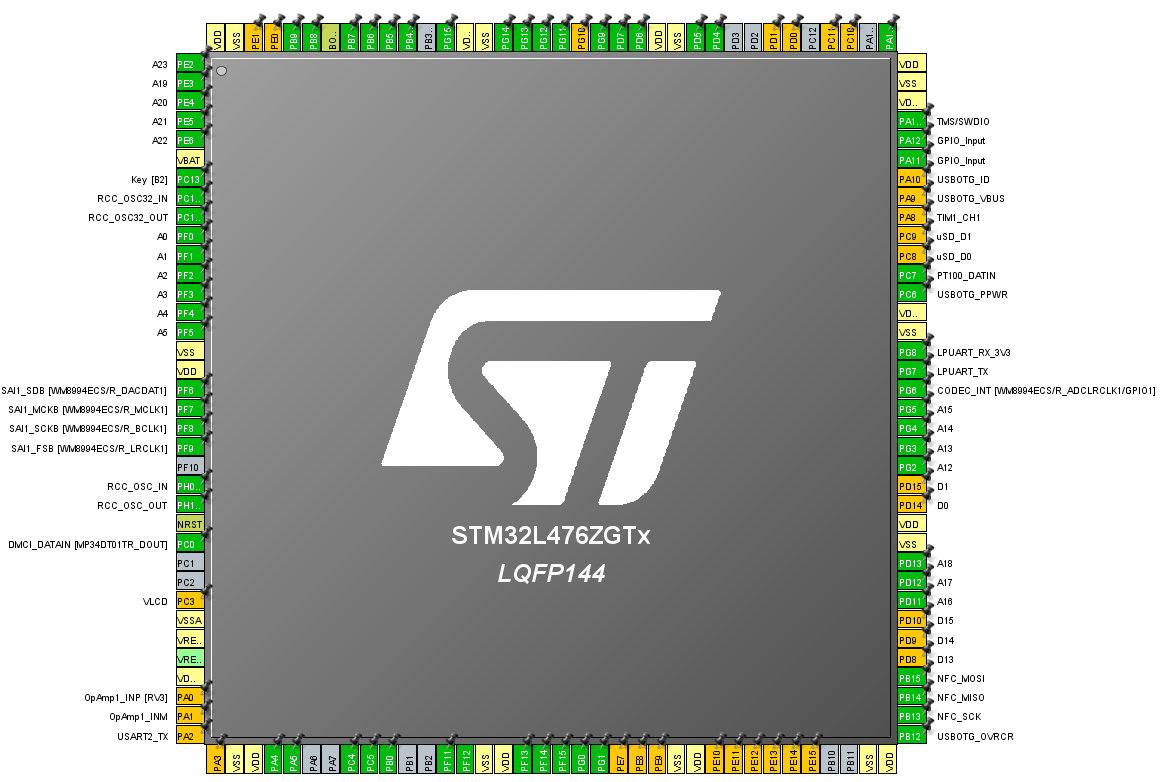
\includegraphics[width=1\textwidth]{figures/piny.png}
	\caption{Konfiguracja wyjść mikrokontrolera w programie STM32CubeMX}
	\label{fig:KonfiguracjaMikrokontrolera}
\end{figure}


\begin{figure}[H]
	\centering
	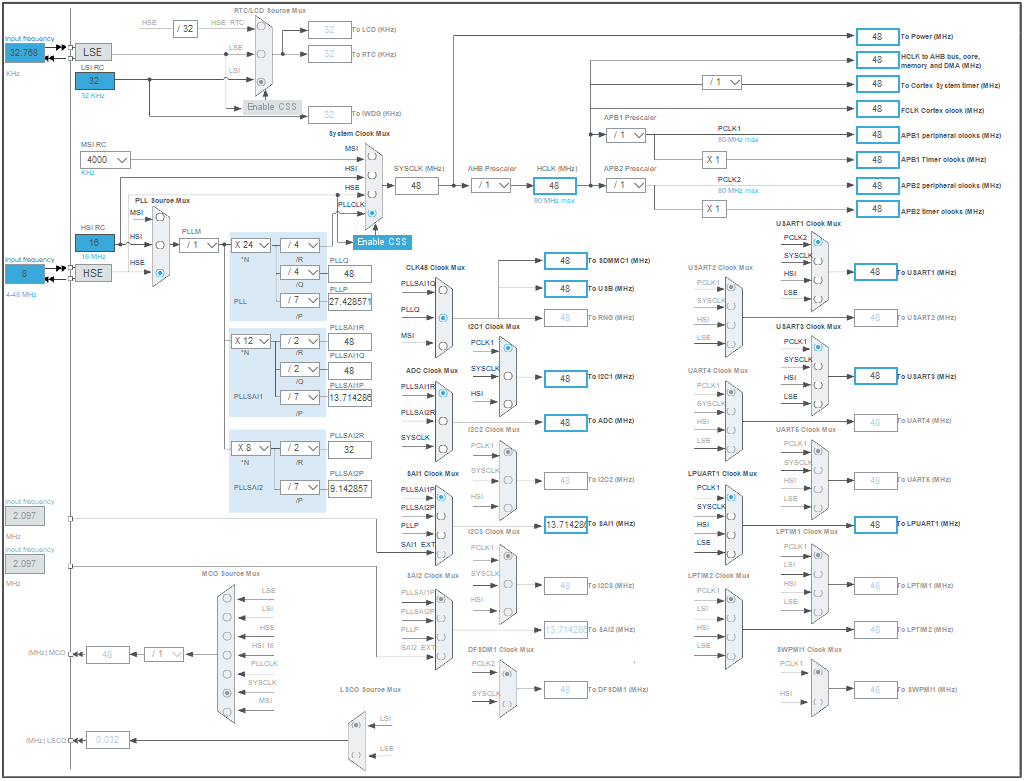
\includegraphics[width=0.9\textheight,angle=90]{figures/zegar.png}
	\caption{Konfiguracja zegarów mikrokontrolera}
	\label{fig:KonfiguracjaZegara}
\end{figure}
\subsection{Konfiguracja pinów}

\begin{table}[H]
	\centering
	\begin{tabular}{|l|l|l|l|}
		\hline
		Numer pinu	&	PIN & Tryb pracy & Funkcja/etykieta\\
		\hline
		8&	PC14 & OSC32\_IN*	RCC\_OSC32\_IN	&\\
		9&	PC15 & OSC32\_OUT*	RCC\_OSC32\_OUT	&\\
		23&	PH0&  OSC\_IN*	RCC\_OSC\_IN	&\\
		24&	PH1&  OSC\_OUT*&		RCC\_OSC\_OUT	\\
		36&	PA2&	USART2\_TX&	USART\_TX\\
		37&	PA3&	USART2\_RX&	USART\_RX\\
		100&	PA8&	TIM1\_CH1&	PWM1\\
		103&	PA11&	GPIO\_Output&	Silnik\_1\\
		104&	PA12&	GPIO\_Output&	Silnik\_2\\


		\hline
	\end{tabular}
	\caption{Konfiguracja pinów mikrokontrolera}
	
\end{table}


%Obecne w dokumencie do etapu I
\section{Harmonogram pracy}

\subsection{Zakres prac}
	\begin{enumerate}
		\item Zapoznanie się z mikrokontrolerem
		\newline
		Wykorzystane to tego celu zostaną poradniki ze strony www.forbot.pl. \cite{kurs1, kurs2, kurs3}
	\end{enumerate}
\subsection{Kamienie milowe}
	\begin{enumerate}
		\item Implementacja działającego prototypu sterowanego joystickiem na płytce.
		\item Implementacja regulacji prędkości w oparciu o regulator PID.
		\item Implementacja sterowania smartfonem.
	\end{enumerate}

\subsection{Wykres Gantta}
Należy wstawić diagram Gantta oraz określić ścieżkę 
krytyczną. Ponadto zaznaczyć i opisać kamienie milowe.

\begin{figure}[H]
	\centering
	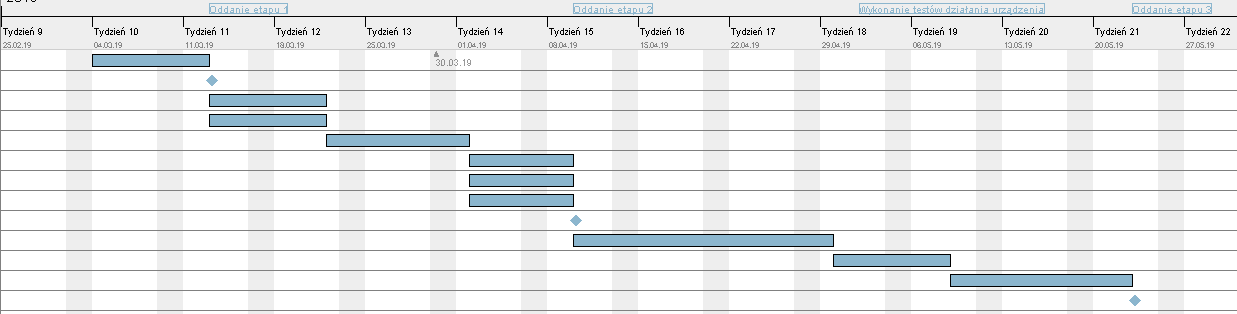
\includegraphics[width=1.1\textwidth]{figures/gant.png}
	\caption{Diagram Gantta}
	\label{fig:DiagramGantta}
\end{figure}

%Obecne w dokumencie do etapu I
\subsection{Podział pracy}

\textbf{Każdy z członków grupy powinien w każdym etapie mieć wymienione od 2 do 4 zadań.}
Przykładowa tabele podziału zadań dla etapu II 
(Tab. \ref{tab:PodzialPracyEtap2}) oraz dla etapu III 
(Tab. \ref{tab:PodzialPracyEtap3})
zostały przedstawione poniżej. 
Przy podziale prac nie uwzględniamy tworzenia dokumentacji projektu!

Przykładowy podział prac:

\begin{table}[H]
	\centering
	\begin{tabular}{|L{7cm}|L{0.8cm}||L{7cm}|L{0.8cm}|}
		\hline
		\hline
		\textbf{Albert Lis} & 
		\% & 
		\textbf{Michał Moruń} & \%\\
		\hline
		\hline
		Schemat elektryczny i elektroniczny		& &	
		Schemat mechaniczny &\\
		\hline
		Budowanie odpowiednich algorytmów & &
		Budowanie odpowiednich algorytmów &\\
		\hline
		Budowa modułu elektronicznego & &
		Budowa modułu mechanicznego & \\
		\hline
		Integracja części mechanicznej oraz elektronicznej & & 
		Integracja części mechanicznej oraz elektronicznej &\\
		\hline
	\end{tabular}
	\caption{Podział pracy -- Etap II}
	\label{tab:PodzialPracyEtap2}
\end{table}

\begin{table}[H]
	\centering
	\begin{tabular}{|L{7cm}|L{0.8cm}||L{7cm}|L{0.8cm}|}
		\hline
		\hline
		\textbf{Albert Lis} & 
		\% & 
		\textbf{Michał Moruń} & \%\\
		\hline
		\hline
		Utworzenie modułu integrującego robota z telefonem & &	
		Utworzenie modułu integrującego robota z telefonem &\\
		\hline
		Integracja ze sobą wszystkich modułów & &
		Integracja ze sobą wszystkich modułów & \\
		\hline
		 Stworzenie interfejsu użytkownika & &
		 Stworzenie interfejsu użytkownika &\\
		\hline
	\end{tabular}
	\caption{Podział pracy -- Etap III}
	\label{tab:PodzialPracyEtap3}
\end{table}



\newpage
%\addcontentsline{toc}{section}{Bibilografia}
%\bibliography{bibliografia}
%\bibliographystyle{plabbrv}
\begin{thebibliography}{9}
	
	\bibitem{kurs1}
	\href{https://forbot.pl/blog/kurs-stm32-f4-1-czas-poznac-hal-spis-tresci-kursu-id14114}{Kurs STM32 F4 z wykorzystaniem HAL oraz Cube}
	\bibitem{kurs2}
	\href{https://forbot.pl/blog/stm32-praktyce-1-platforma-srodowisko-id2733}{Kurs STM32 F1 z wykorzystaniem bibliotek STDPeriph}
	\bibitem{kurs3}
	\href{https://forbot.pl/blog/kurs-stm32-f1-migracja-na-hal-wstep-spis-tresci-id23580} {Kurs STM32 F1 z wykorzystaniem bibliotek HAL}
		\bibitem{kurs4}
	\href{https://media.readthedocs.org/pdf/arduino-esp8266/docs_to_readthedocs/arduino-esp8266.pdf} {ESP8266 Arduino Core Documentation}
			\bibitem{kurs5}
	\href{https://docer.pl/doc/n5xcex8} {Teoria sterowania w ćwiczeniach}
	
\end{thebibliography}


\end{document}







































